% -- Encoding UTF-8 without BOM
% -- XeLaTeX => PDF (BIBER)

\documentclass[]{cv-style}          % Add 'print' as an option into the square bracket to remove colours from this template for printing. 

\sethyphenation[variant=british]{english}{} % Add words between the {} to avoid them to be cut 

\begin{document}

\header{}{Emily Quinn Finney}           % Your name
%\lastupdated

%----------------------------------------------------------------------------------------
%	WORK EXPERIENCE SECTION
%----------------------------------------------------------------------------------------

\section{Data Experience}

\begin{entrylist}
%------------------------------------------------

\entry
  {2015-2017}
  {Graduate Research Associate}
  {Davis, CA}
  {\jobtitle{University of California, Davis} 
  \begin{itemize}
    \item Trained high-dimensional models of galaxy cluster structure using MCMC and gradient descent algorithms. 
    \item Extracted wavelength information and other properties from imaging data.
    \item Wrote a peer-reviewed journal article detailing results.
    \item Provided extensive mentoring in astrophysics research practices.\\
  \end{itemize}}
\entry
  {2013}
  {Undergraduate Senior Thesis}
  {Claremont, CA}
  {\jobtitle{Scripps College} 
  \begin{itemize}
    \item Implemented Bayesian methods to improve models of galaxy cluster mergers.
    \item Inferred galaxy cluster collision parameters by analyzing radio data.
    \item Visualized data and communicated findings in a paper.
    \item Selected to present research at Scripps College Capstone Day.\\
  \end{itemize}}
\entry
  {2013}
  {Astronomy Research Internship}
  {La Serena, Chile}
  {\jobtitle{Cerro Tololo Inter-American Observatory}
  \begin{itemize}
    \item Cleaned gigabytes of astronomical data using bash scripting and Skycat image software.
    \item Classified spectral data and fit lines to redshifts.\\
  \end{itemize}}
\entry
  {2012}
  {Physics Research Internship}
  {Davis, CA}
  {\jobtitle{University of California, Davis}
  \begin{itemize}
    \item Conducted hypothesis testing on a set of galaxy ellipticity data.\\
  \end{itemize}}

%------------------------------------------------

\end{entrylist}


%----------------------------------------------------------------------------------------
%	SKILLS SECTION
%----------------------------------------------------------------------------------------

\section{Teaching Experience}
\begin{entrylist}
%------------------------------------------------

  \entry
      {2017}
      {Elementary Math/Science Teacher}
      {Davis, CA}
      {\jobtitle{The Peregrine School}
        \begin{itemize}
        \item Managed a classroom of 20 students ages 8-12.
        \item Designed and implemented project-based lesson plans to convey physics, math, and computer programming concepts.\\
          \end{itemize}}
\entry
  {2014-2016}
  {Physics Teaching Assistant}
  {Davis, CA}
  {\jobtitle{University of California, Davis}
  \begin{itemize}
    \item Taught physics discussion/labs for 40-60 students each academic quarter.
    \item Responsible for weekly office hours, grading, and proctoring exams.\\
  \end{itemize}}
\entry
  {2012-2014}
  {Physics and Computer Science Tutor/Grader}
  {Claremont, CA}
  {\jobtitle{Scripps College; Harvey Mudd College}
  \begin{itemize}
    \item One-on-one tutoring in physics and computer science concepts.\\
  \end{itemize}}
%\entry
%  {Summers}
%  {Camp Director}
%  {Davis, CA; Reno, NV; Plymouth, MA}
%  {\jobtitle{The Peregrine School; Great Basin Institute; Camp Clark YMCA}
%  \begin{itemize}
%    \item Designed and implemented physics, ecology, and computer programming oriented curricula for students ages 4-16.\\
%  \end{itemize}}
%------------------------------------------------

\end{entrylist}

%----------------------------------------------------------------------------------------
%	EDUCATION SECTION
%----------------------------------------------------------------------------------------

\section{Education}

\begin{entrylist}
%------------------------------------------------
\entry
{2014--2017}
{Master's of Science, Physics}
{Davis, CA}
{\jobtitle{University of California, Davis}}

{\vspace{-0.2cm}}
\end{entrylist}
%------------------------------------------------
\begin{entrylist}
\entry
{2010--2014}
{Bachelor's of Arts, Physics}
{Claremont, CA}
{\jobtitle{Scripps College}}
\end{entrylist}

%----------------------------------------------------------------------------------------
%	INTERESTS SECTION
%----------------------------------------------------------------------------------------

\section{Other Skills and Interests}
  \vspace{-0.2cm}

  \textbf{Professional} \hspace{0.05cm} Machine learning, tidy data, image analysis, data-driven education. \\
  \textbf{Personal} \hspace{0.57cm} Hiking, child development, spiders, theology, singing.
  
%----------------------------------------------------------------------------------------

%----------------------------------------------------------------------------------------
%	SIDEBAR SECTION  -- In the aside, each new line forces a line break
%----------------------------------------------------------------------------------------

\begin{aside}
%
\section{Software}
\textbf{Python}
%{\color{red} $\varheartsuit$} 
NumPy\\ SciPy\\ Pandas\\ matplotlib
%\LaTeX{}
\textbf{Unix/Linux}
bash scripting
Git
\textbf{Software Design}
OOP
C data types
\textbf{R}
tidyverse enthusiast
\textbf{Other Languages}
Java\\ MATLAB\\ SQL\\ \LaTeX
%
\section{Practical Statistics}
\textbf{Bayesian Methods}
Bayes' Theorem
MCMC
\textbf{Statistical Inference}
Random variables
Hypothesis testing
Regression
Experimental design
\textbf{Machine Learning}
Gradient descent
Clustering algorithms
\textbf{Mathematics}
Linear algebra
Multivariate calculus
%
\section{Photo}
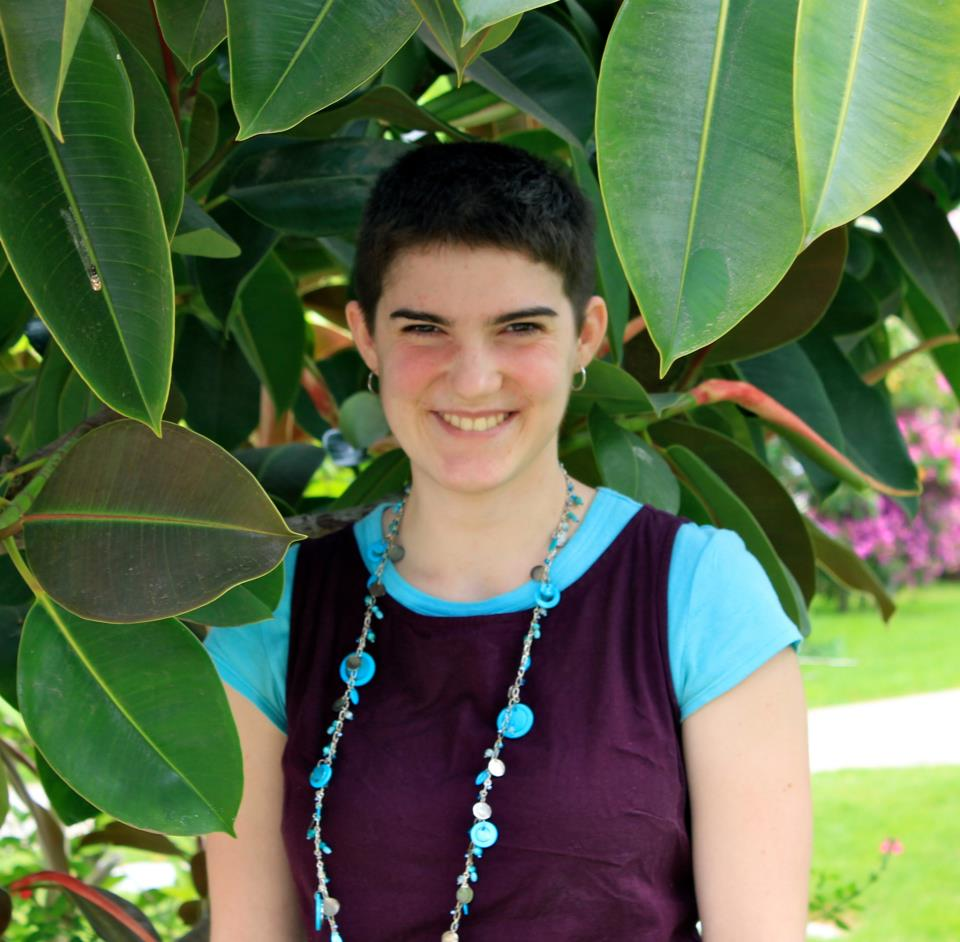
\includegraphics[width=3.6cm,height=3.6cm]{headshot.jpg}
%
\section{Contact}
549 Commercial Ave Apt. 6\\ South San Francisco, CA \\\hspace{0.5cm}94080
%
eqfinney@\\\hspace{0.5cm}ucdavis.edu
%
(339) 933-3936
%
linkedin.com/in/\\\hspace{0.5cm}emily-quinn-finney
%
github.com/eqfinney
%
\end{aside}

\end{document}
